\documentclass[12pt]{report}
\usepackage[utf8]{inputenc}
\usepackage{graphicx}
\usepackage{geometry}
\geometry{margin=1in}
\usepackage{fancyhdr}
\pagestyle{fancy}

\usepackage{float}
\usepackage{amssymb}
\usepackage{amsmath}
\usepackage{amsthm}
\usepackage{ulem} 

\usepackage{caption}
\usepackage{subcaption}

\usepackage{titlesec}
\usepackage{setspace}
\usepackage{hyperref}
\usepackage[labelfont=bf, textfont=md]{caption}

\usepackage[square,numbers]{natbib}
\usepackage{indentfirst}

\title{
	\Huge{Modeling the mechanisms of dynein's step using Monte Carlo simulations and Brownian dynamics}\vspace{1em}\\
	\Large{Jin Kiatvongcharoen} \vspace{0.5em}\\ 
	\normalsize{Department of Physics, Oregon State University}\vspace{2em}\\
	
\includegraphics[width=0.4\columnwidth]{OSU_logo.png}\vspace{1em}\\
	\normalsize{An undergraduate thesis advised by Dr. David Roundy}\\
	\normalsize{in partial fulfillment of the requirements for the degree of}\\
	\normalsize{Baccalaureate of Science in Physics}\vspace{1.5 em}\\
	\normalsize{Submitted \today}\\


}
\date{}

\begin{document}
    \maketitle
    \onehalfspacing


	\chapter*{Abstract}
	Molecular motor proteins are responsible for the cell’s ability to move, divide, and spatially organize itself. A defect within any of the three motor proteins can cause severe damage to the cell’s functionality and lead to neurological diseases. In order to fully understand the cause of such possible diseases, the motor protein dynein and more specifically its structure has been extensively studied. However, there has been limited research focused on the motion of dynein. To investigate this, we will simulate dynein’s stepping mechanisms using Monte Carlo methods and Brownian dynamics. The dynein will be computationally replicated with a particle-rod model undergoing Brownian motion in a fluid, where its stepping will be repeatedly simulated to generate an ensemble of statistics, via the Monte Carlo. The program will optimize dynein’s stepping patterns by fitting parameters according to experimental results of dynein’s step length, time, and probability of stepping. 
	
    \begin{spacing}{1.2}
	\tableofcontents
	\listoffigures
	\end{spacing}
	
	
	\chapter{Introduction}
	%\textit{Introduce topic by talking about cells. Attention grabber, relate biophysics study to cancer reserach and many areas where we need to focus our research. Short and sweet, maybe 1 or 2 short paragraphs.}

	Neurodegenerative diseases, such as Alzheimer's and Huntinton's disease, have consistently been one of the leading causes of death in the United States \cite{eschbach2011cytoplasmic}. Scientists all over the world struggle to find a solution for these diseases and continue to hope for a breakthrough in science in attempt to prevent or even cure these fatal diseases. Although this breakthrough has yet to come, research suggests that motor protein failure is a main cause of cell degeneration. More specifically, defects in the motor protein dynein have been linked to neurodegeneration due to the cell's funtional dependence on dynein and its mechanical properties. However, unlike dynein's motor protein siblings, dynein possesses a unique structure causing it to stochasitcally move around the cell and be unpredictable in nature. Thus, fully understanding the mechanisms of dynein can allow us to further understand causes of its failure. In this paper, we propose a model of dynein that uses Monte Carlo methods and a Brownian dynamics simulation to reproduce dynein's unique steping behavior. What follows is a brief introduction to the dynein motor protein, a review of the powerstroke model, and the framework for a computational simulation of the powerstroke, which we seek to replicate Yildiz's observation of correlated stepping.  

\section{Background}

\begin{figure}[H]
	\centering
	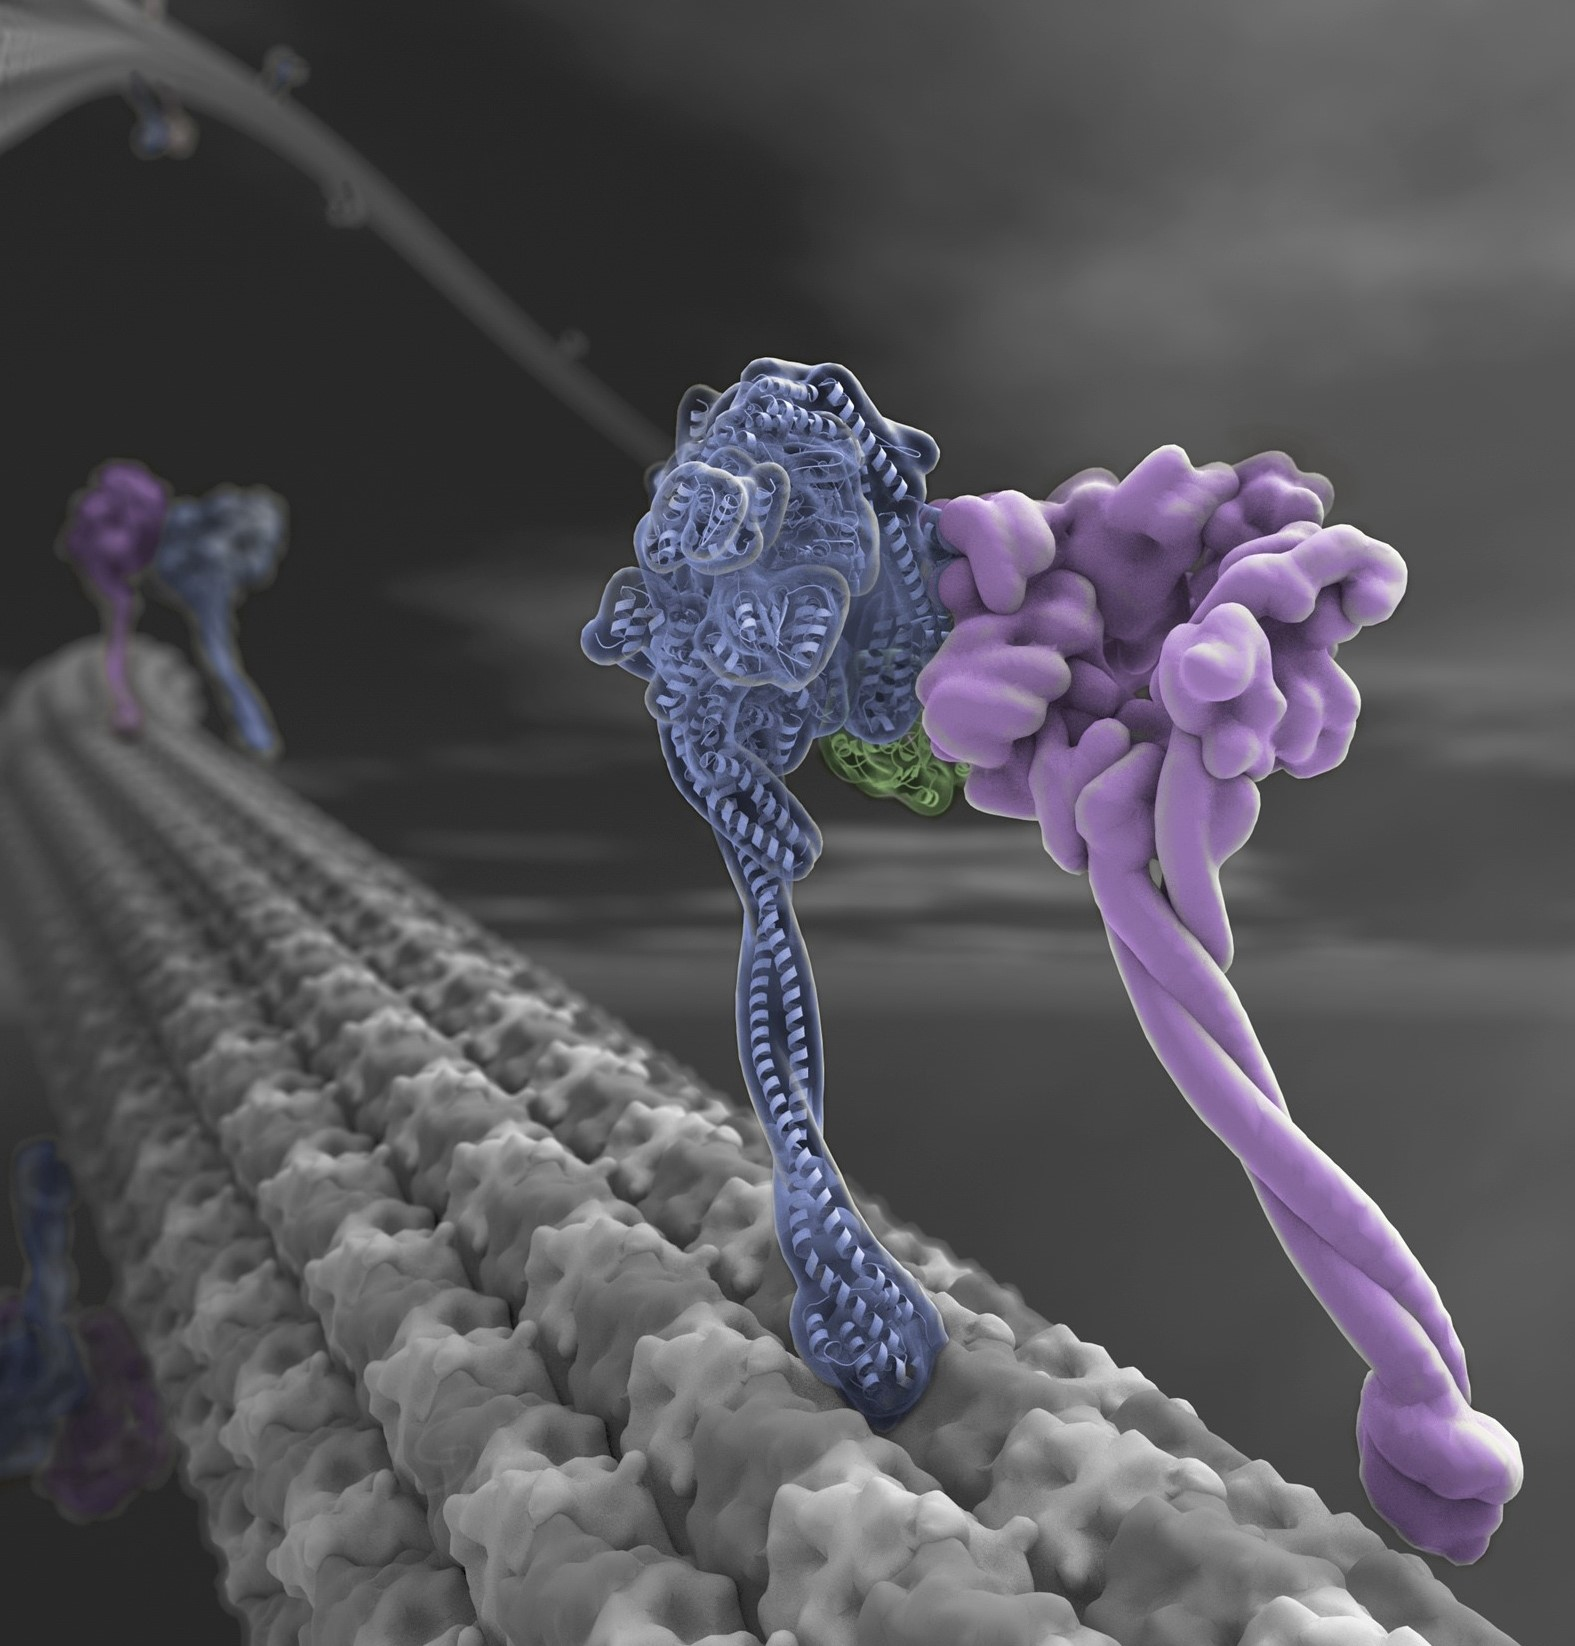
\includegraphics[width=0.5\columnwidth]{Figures/dynein_walking_art.jpg}
	\caption[Artist Rendition of Dynein]{\textbf{Artist Rendition of Dynein} walking along a microtubule in a cell. \cite{JohnsonArt}}
	\label{fig:ArtDynein}
\end{figure}

Cells are complicated. They have the ability to move, perfectly divide, and spatially organize themselves when they are functional, but can also be responsible for death when they are not. They can function because tiny, two-legged molecular proteins, named \textit{motor proteins}, carry cargo with information around the cell. These motor proteins are kinesin, myosin, and dynein. They travel around the cell on a cytoskeleton composed of microtubules (MT) that act as a walkway for the proteins. A depiction of dynein walking along the microtubule is shown above in Figure (\ref{fig:ArtDynein}). Microtubules are constructed from negatively charged $\alpha$- and positively charged $\beta$-tubulin dimers that polarize the microtubule depending on which tubulin is left hanging at the ends. In a eukaryotic cell, microtubules typically stem outwards from the cell's nucleus to the cell walls where the $\beta$ tubulin is exposed, generating a positive end that pulls kinesin and myosin. However, dynein walks toward the nucleus cell body where the MT is negatively charged. This attraction to drives the directed stepping motion for each motor protein and is shown in Figure (\ref{fig:transport}). 

\begin{figure}[H]
	\centering
	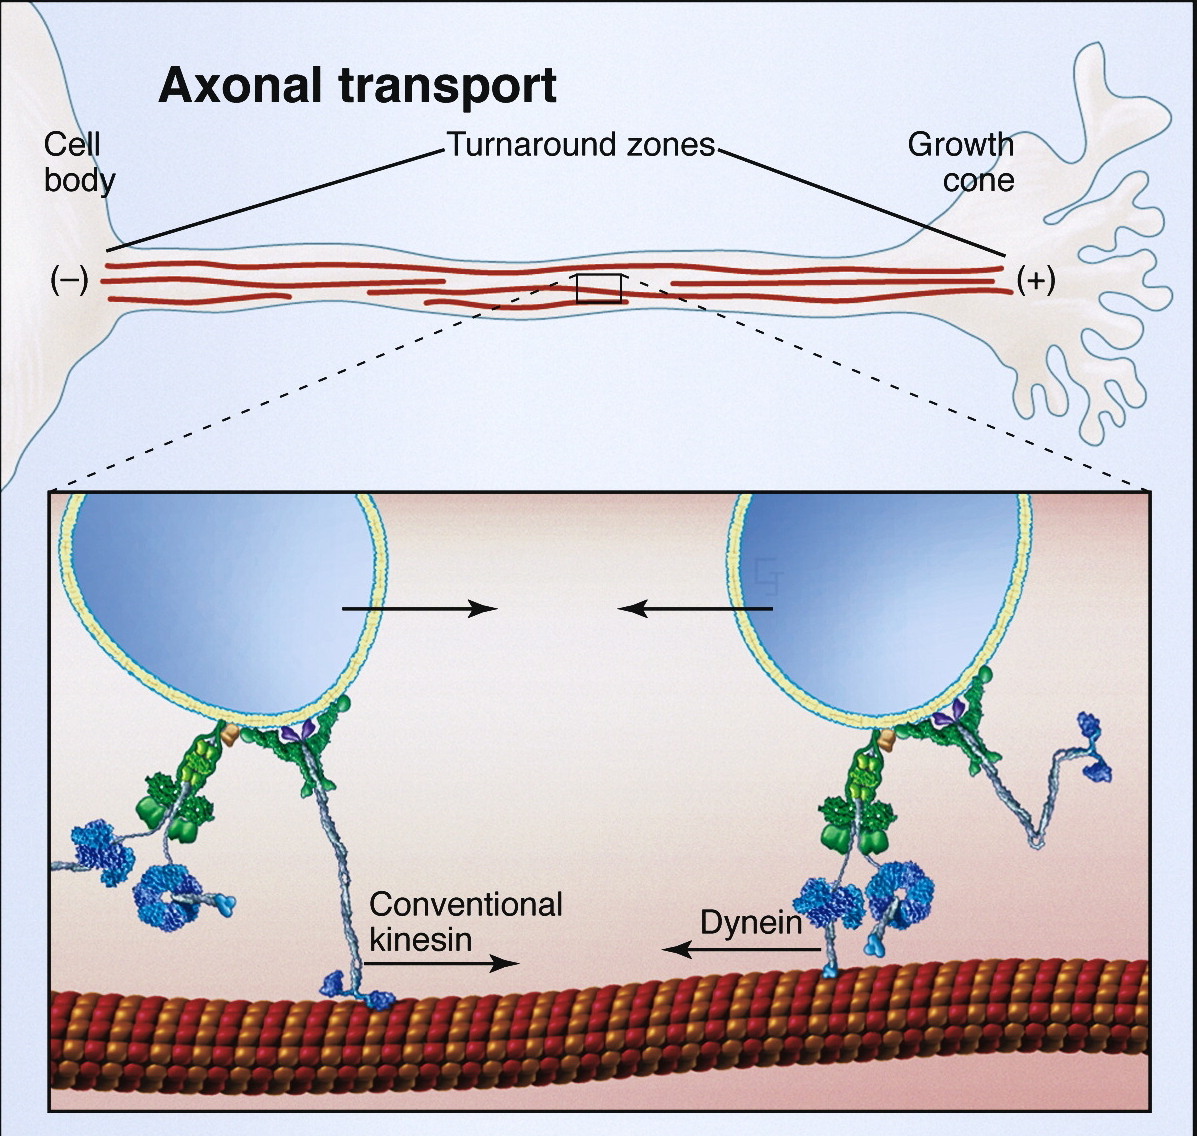
\includegraphics[width=0.6\columnwidth]{Figures/retrograde_transport.jpg}
	\caption[Charge Influenced Transport]{\textbf{Charge Influenced Transport}. Dynein and kinesin transporting cargo on the axon of a neuron cell for building the axon growth cone. They share cargo and take turns delivering each other to opposite ends of the cell. \cite{Vale2003molecular}}
	\label{fig:transport}
\end{figure}

Both kinesin and myosin exhibit hand-over-hand stepping, where their ``legs" take turns alternating steps like a human. Due to dynein's massive size compared to its motor protein siblings, dynein does not step uniformly but rather inchworms its ``feet" like a drunk human. This unique property makes dynein difficult to study when analyzing possible sources of molecular failure, but illustrates the importance of understanding the physical structure of the entire motor protein.

\section{Structure}
%\textit{In-detail background knowledge on structure of dynein. Talk about each domain and their roles. Binding domain, six AAA+ domains, tail, and cargo. Stalk and linker that attaches things together. How the structure is so much larger than that of kinesin. dynein has flexibility because of its linker and in order to compensate for its huge domains. }

Dynein is composed of two motor heavy chain subunits of linked amino acids, called polypeptides, each which are separated into domains. Figure (\ref{fig:structure}) displays these domains and labels them as the tail domain, motor domains (constructed from six AAA+ domains that form a ring), and the microtubule binding domains. The tail and the motor domains are connected by separate linkers, while the motor and the binding domains are connected by the stalks.

%\begin{figure}[H]
%	\centering
%	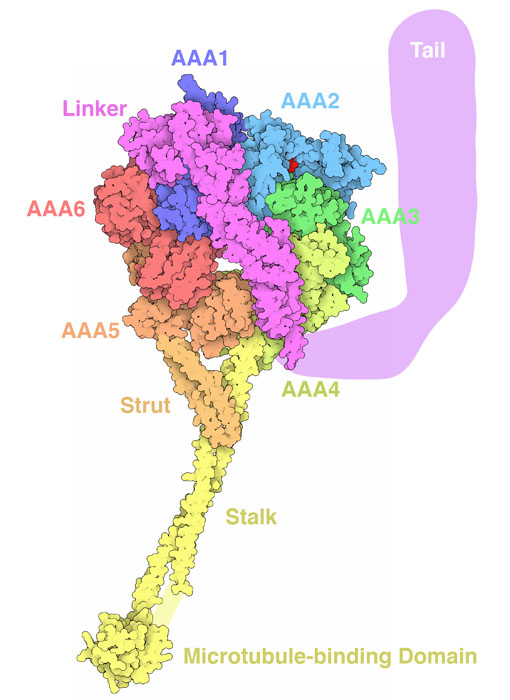
\includegraphics[width=0.6\columnwidth]{Figures/dynein_polypeptide.jpg}
%	\caption[Polypeptide Structure]{\textbf{Polypeptide Structure} \cite{GoodsellArt}}
%	\label{fig:polypeptide}
%\end{figure}

\begin{figure}[H]
	\centering
	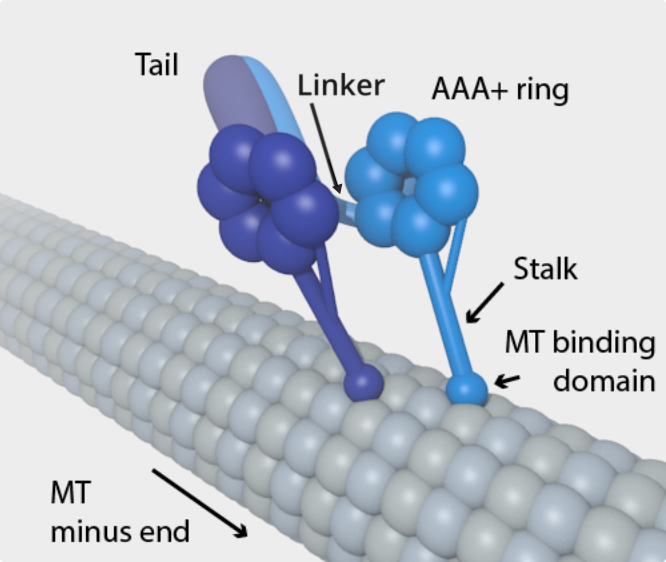
\includegraphics[width=0.6\columnwidth]{Figures/dynein_on_MT.png}
	\caption[Structure of Dynein]{\textbf{Structure of Dynein.} Illustration of cytoplasmic dynein's heavy chain subunits bounded to the microtubule. The AAA+ rings block the view of the independent linkers connecting to the tail. This rendition depicts dynein’s structure as a domain-rod system. \cite{TheTrappistArt}}
	\label{fig:structure}
\end{figure}

Dynein's crystal structure has been rigorously studied because of the pivotal role it plays in dynein's unpredictable stepping nature. Its inability to step uniformly is largely due to the large lengths between each major domain site, as the linker and stalk are about a factor of a half larger than the diameter of the AAA+ ring. In kinesin and myosin, the motor domains are much closer to the MT, causing a more controlled and consistent step due to their low center of mass. Despite dynein's large structure, it can still achieve processive stepping due to the interaction of adenosine triphosphate (ATP) with the AAA+ domains, which is why the AAA+ domains are referred to as the motor domains.





\section{Stepping}
%\textit{Biology and chemistry of stepping. What is actually causing it to step? ATP hydrolysis. Maybe short introduction on stepping and go more in detail in Power Stroke model. Say there are multiple theories and models of how dynein steps. Powerstroke, Winch, etc. Power stroke is most accepted. It can step on microtubule that is made up of tubulin dimers, $\alpha$ and $\beta$ tubulins. They are normally 8nm apart and so experimentalists believe dynein average step is always factor of 8nm. }

Dynein's ability to step is entirely ATP driven under the process of ATP hydrolysis. The ATP binds to the motor domain and converts chemical energy into mechanical energy for the dynein to transition between differenet conformational states during a step. This process allows the binding domains to let go and reattach to the microtubule at different locations causing varying step sizes. We can measure dynein's step length by definining an axis on the microtubule for where dynein can step.

The on-axis is defined to be the axis parallel to the direction of forward stepping towards the negative end of the microtubule, while the off-axis is defined to be the axis perpendicular, as shown in Figure (\ref{fig:axis}). Figure (\ref{fig:axis}) also displays the alternative helix structure of the $\alpha$- and $\beta$-tubulin dimers, in which act as the landing zones for dynein's binding domain.  

\begin{figure}[H]
	\centering
	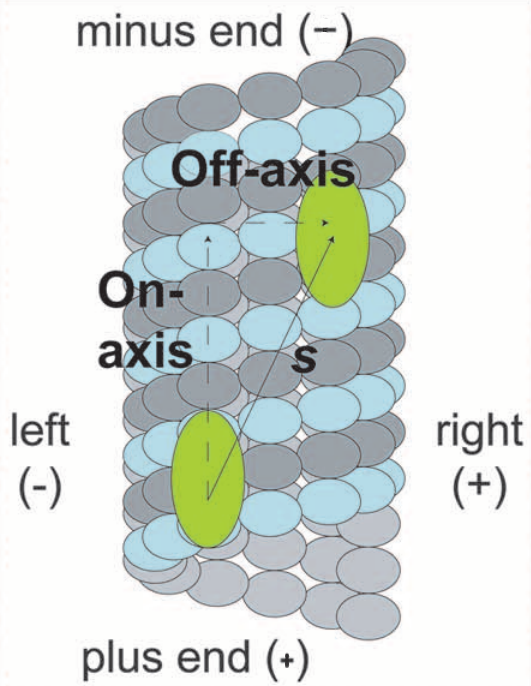
\includegraphics[width=0.3\columnwidth]{Figures/Onaxis.png}
	\caption[Stepping Axis]{\textbf{Stepping axis.} Birds-eye view of the microtubule with the green areas identifying the microtubule binding domains. For the on-axis, positive displacement is defined towards the minus end of the microtubule. Dark grey and light blue helix structure indicates $\alpha-$ and $\beta-$tubulin dimers. \cite{Dewitt2012} }
	\label{fig:axis}
\end{figure}

While ATP hydrolysis dictates the forward stepping during dynein's walk, the geometry of the domains is still a question for experimentalists. How exactly do the motor, tail, and linker achieve processive motion? Do the motor domains act as knees and stretch out for a step? Or do the knees stay bent, while the tail swings forward? Despite ongoing debates, researchers suggest the former and named this process the powerestroke model. 



\subsection{Powerstroke Model}
%\textit{Theorized model of stepping. Mechanochemical Cycle. Talk about ATP hydrolysis. Different conformational changes within a step. Look at linker and how it changes angles. Physically, it looks like it unbinds, stretches leg, then kicks forward, then diffuse back to MT.} 

The widely accepted powerstroke model was best exhibted within the mechanochemical cycle introduced by Cianfrocco et al. \cite{Cianfrocco2015mechanism}. A summary of the eight step cycle is shown below in Figure (\ref{fig:MechanochemicalCycle}).

\begin{figure}[H]
	\centering
	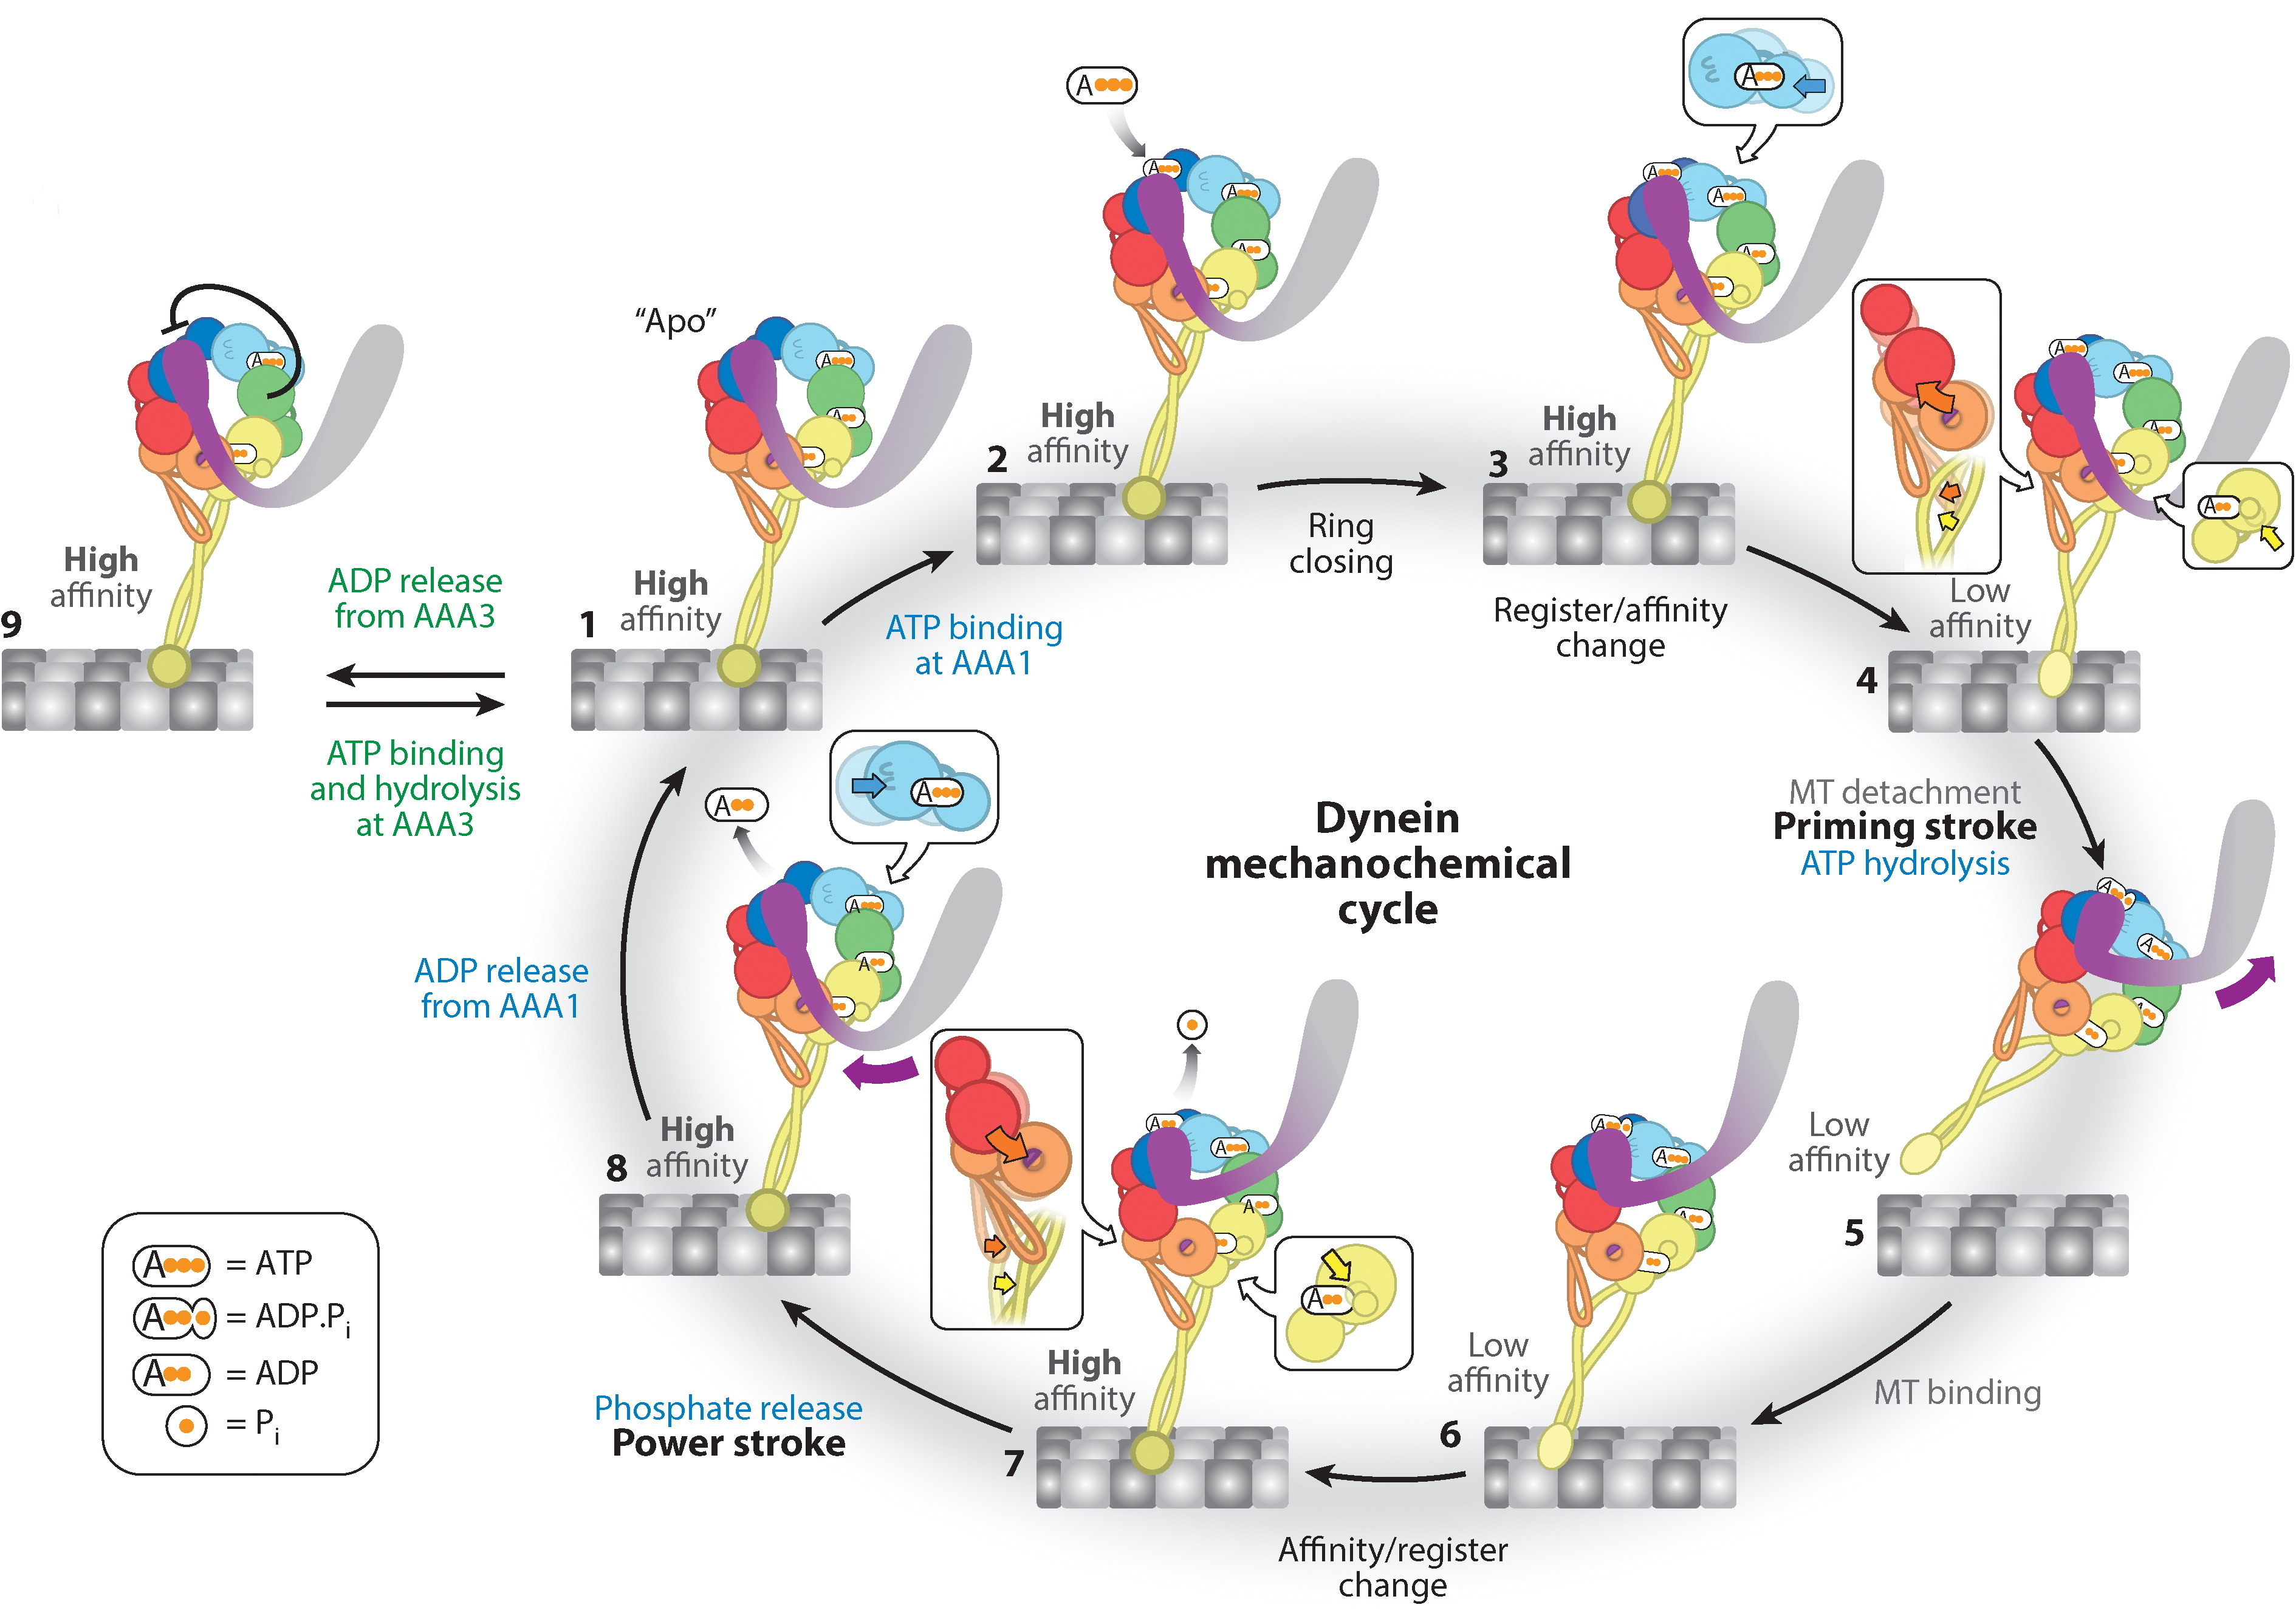
\includegraphics[width=1\columnwidth]{Figures/mechanochemical_cycle.jpeg}
	\caption[Mechanochemical Cycle]{\textbf{Mechanochemical Cycle.} The proposed series of conformational stages dynein undergoes during a step. The interaction of ATP with the motor domain is the main factor causing the powerstroke.  \cite{Cianfrocco2015mechanism}}
	\label{fig:MechanochemicalCycle}
\end{figure}

The cycle utilizes the conformational transition between high affinity and low affinity to explain dynein's unbinding and rebinding process. This transition is governed by the addition of an ATP unit, which loosens the ``foot" from the MT (steps 3 to 4), stretches the linker (steps 5 to 6), and tightens the ``foot" back onto the MT (steps 6 to 7), pulling the whole protein forward. This key detail within the transition of stretching the linker distinguishes a ``pre-" and a ``post-" stroke state during the powerstroke model and can be analogous to bending a knee upwards and kicking the foot forwards to stretch the knee and take a step. A closer visualization of this transition between pre- and post-stroke states can be seen in Figure (\ref{fig:Powerstroke}), where the linker is highlighted in yellow.  

\begin{figure}[H]
	\centering
	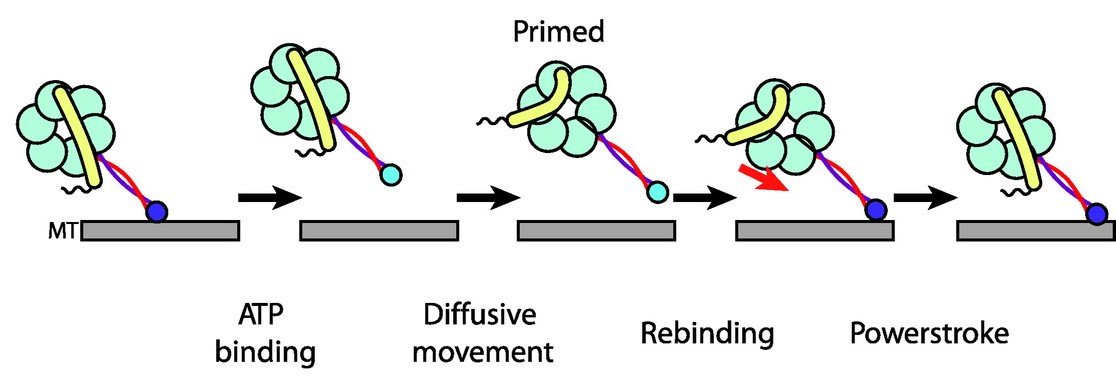
\includegraphics[width=1\columnwidth]{Figures/powerstroke.jpeg}
	\caption[Powerstroke]{\textbf{Powerstroke.} A more detailed visualization of the linker during the transition from pre- to post-stroke states. The linker is initially bent inwards during the pre-stroke state, then stretches backwards to extend the binding domain forward and land during the post-stroke state. \cite{Carter2010communication} }
	\label{fig:Powerstroke}
\end{figure}

Although the mechanochemical cycle provides a reasonable model for dynein's step and illustrates the motion between the domains, the model still generalizes the dependencies of the step and fails to analyze different geometric factors that can alter the conformations.


\section{Experimental Research on Dynein}

Experimental research investigates the correlations within dynein's stepping pattern and how different parameters may affect the step. These consists of the angle dependency during the stretching of the linker, the affect of the initial conformation when taking a step, the ATP concentration for hydrolysis, etc. However, due to dynein's small scale, experiment often disagrees with one another and differs depending on the technique of measuring dynein. 

%Although the mechanochemical cycle provides a reasonable model for dynein's step, the model fails to analyze the precise movements of each domain and how different configurations alter the conformational transitions. To what extent does the linker stretch when exhibiting the powerstroke and is it angle dependent? How does the separation between the two subunits of dynein affect the step length of the powerstroke? Consequently, these questions inspire experimentalists to measure dynein's step and study correlations between different parameters within a step.

\subsection{Measuring}
%\textit{How are experimentalists measuring dyneins stepping? Quantum dots on motor domains or quantum rod on tail, etc. }

Experimentalists approach measuring dynein in various ways, which can involve electron microscopy or quantum measuring techniques. Some attach quantum dots to dynein's motor domains, while others replace the tail with an artificial quantum rod. Despite the different procedures, all measuring techniques suffer from their inability to measure small (\textit{change word}) movement. This causes steps with short step lengths to be undetectable, such as if dynein quickly rebinds at the same spot after unbinding. The various measuring procedures and experimental limitations leads to different results and unique findings when observing different variables. In this paper, we will focus on Yildiz et al. unique finding of observing a stepping correlation between the initial interhead separation and step length. 


\subsection{Yildiz's Stepping Correlation}
%\textit{Purpose of my research. Trying to make model and fit to Yildiz analysis of dynein having interstep correlation. Dependency between step length and initial inter head separation.}

Dynein's large size and stochastic nature implies completely independent stepping from the initial conformational state before the step. However, in 2012, Yildiz et al. observed a correlation between the initial on-axis separation and the step length, indicating a dependence on the interhead separation \cite{Dewitt2012}. This discovery challenged established views on dynein's stepping processivity and pose the question of whether there exists interhead coordination between the motor domains when stepping. Figure (\ref{fig:YildizCorrelation}) below displays this correlation with a linear regression where an existing non-zero slope indicates a dependence between the step and the initial on-axis separation.

\begin{figure}[H]
	\centering
	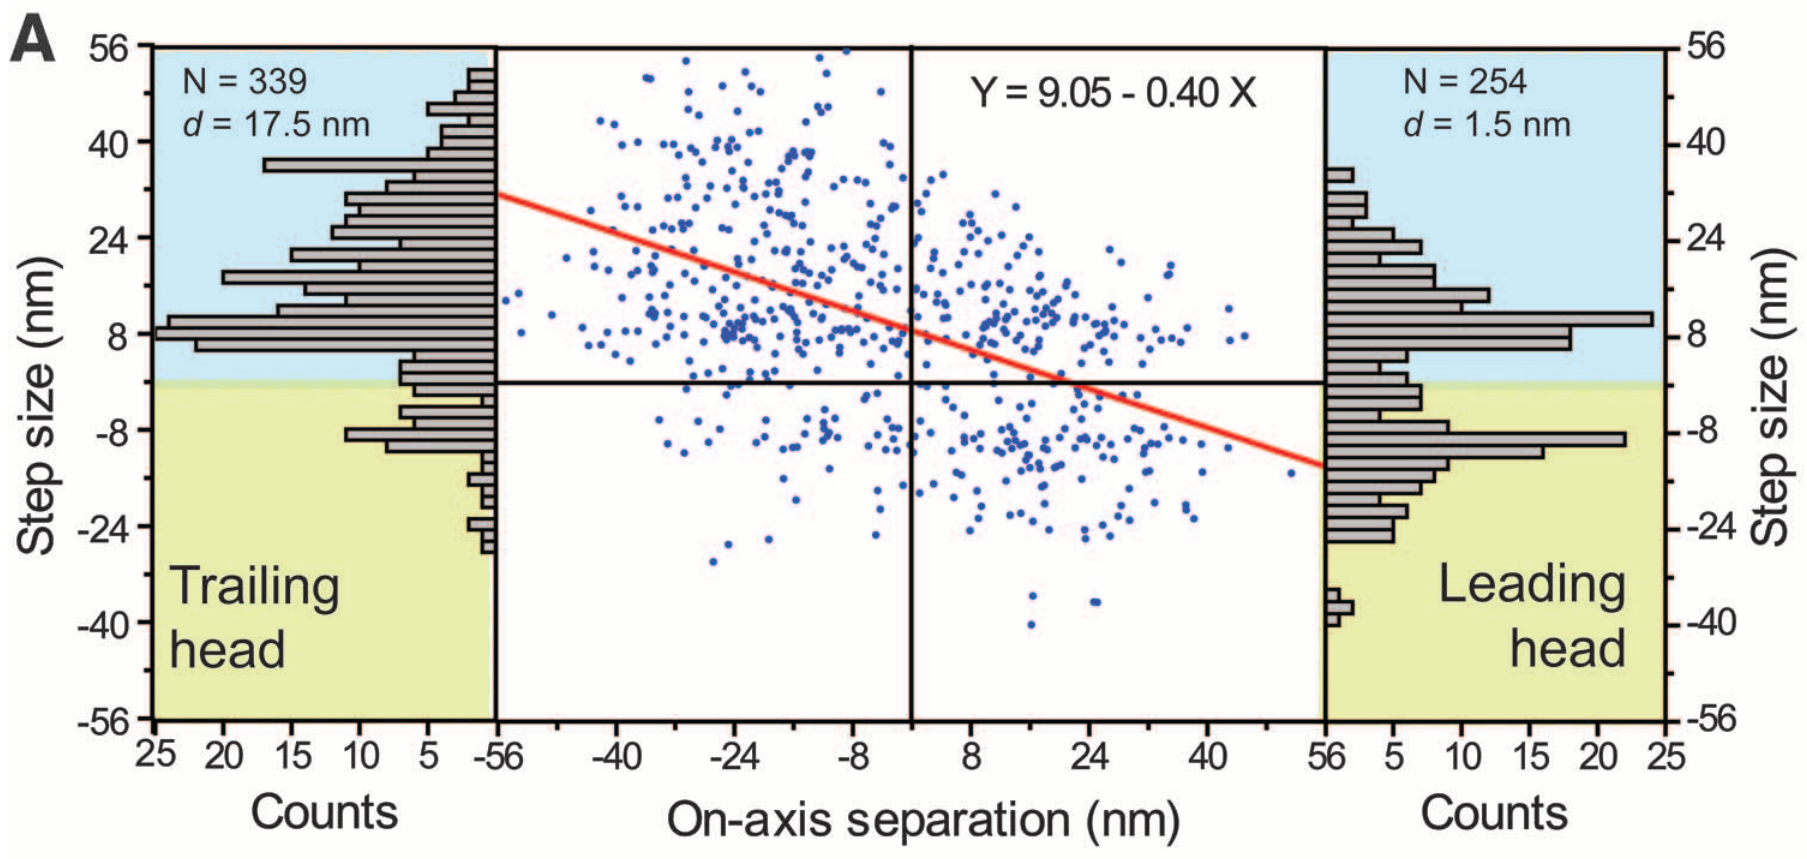
\includegraphics[width=1\columnwidth]{Figures/Yildiz_stepping.png}
	\caption[Stepping Correlation]{\textbf{Stepping Correlation.} A scatter plot of step sizes vs. on-axis separation which hints at a functional dependency between the step  length and the initial distance between the binding domains. The 1D histogram for the trailing head on the left only generalizes the step lengths for negative on-axis separation, while the histogram for the leading head does the same for positive on-axis separation. \cite{Dewitt2012} }
	\label{fig:YildizCorrelation}
\end{figure}

This correlation implies a connection between the physical state of dynein and its stepping behavior, inferring that dynein's step is not only ATP dependent. Unfortunately, experiment is inherently limited and can massively benefit from accurate models that can simulate dynein's stepping under realistic circumstances.


\section{Motivation}
%\textit{Briefly write about the importance of dynein, how dynein is researched when studying neurological diseases, dynein stepping is understudied compared to other motor proteins, hard to model dynein because of random walking, there are almost no computational models of dynein that uses molecular dynamics, modelling dyenin can give us better understanding of why it moves the way it does, specific motivation for model: new research found that there is interhead coordination when stepping so maybe we can use that to base our model off of.}

We want to further investigate Yildiz's unique stepping correlation by creating a compuational simulation of dynein and analyze the specific conditions that are required to replicate their results. Currently, other simulations that model dynein's step exist, but all of them are used to investigate the ATP hydrolysis mechanism during the mechanochemical cycle. These simulations suffer from numerous assumptions made about the physical aspects of dynein's step. (\textit{Should reference a simulation here}) Some assume that dynein can step only in increments of 8nm or that the rebinding process is constrained to a certain time frame. These limitations make it impossible for the models to replicate unique discoveries about dyneins stepping, such as Yildiz's correlation from above.

To bridge this gap, Roundy et al. constructed a physical model of dynein that explores the molecular interactions between the domains of dynein and its aqueous environment. Instead of making assumptions about the physical properties of the step, Roundy's model neglects the chemistry of the ATP exchange and assumes that the energy transfer from the ATP is incorporated within the binding processes. Researchers John Waczak and Elliott Capek successfully incorporated this model under an angle-dependent Brownian dynamics simulation, where each domain experiences Brownian motion during a step to mimic stochastic movement \cite{Capek2017, }. They were able to track dynein's precise movement along a walk and compare their stepping results to experiment. However, their simulation suffered from immense computaiton time and lacked the ability to optimize model parameters for a better fit to experiment. For this work, we will use their simulation as a foundation and implement a Monte Carlo method for reproducing data fast and generating an ensemble of statistics. We intend to use this model to reproduce experimental measures and help verify existing understandings concerning the properties of dynein’s stepping mechanism. More specifically, we want reproduce Yildiz's unique findings and investigate the stepping dependence on the interhead separation. 



%\textit{THIS IS STRAIGHT FROM PROPOSAL, NEED TO FIX THIS AND ADJUST SO THAT MORE DYNEIN DETAILS GOES INTO CHAPTER 2}
%
%In a eukaryotic cell, dynein is one of the three motor proteins that are responsible for the cell’s ability to move, divide, and spatially organize itself. Similar to the more researched kinesin, dynein conveys cargo along the microtubule track by using ATP to power its two binding domains (its “feet”). However, its walking-like movements along the track are very unpredictable and can vary in terms of distance and direction. Dynein’s two feet can also act independently from each other causing much more erratic and stochastic steps. However, despite dynein’s stochastic nature, dynein is still able to achieve processive motion due to the functions of its structure. Structurally, dynein is composed of two motor heavy chain subunits of linked amino acids, called polypeptides, each which are separated into domains. These domains are the tail domain, the linker domain, the six AAA+ domains, and the microtubule binding domains (See Figure 1). The AAA+ domains are responsible for ATP hydrolysis, in which converts chemical energy stored in ATP into mechanical work causing dynein’s motility. 
%
%Because dynein’s stepping is unpredictable in nature, its stepping mechanism has not been intensely studied as compared to its structure. Questions regarding the electrostatic interactions with the microtubule, ring stacking, discrete microtubule binding sites, or elasticity of the stalk are yet to be answered. A known and supported model to describe dynein’s motion is the powerstroke model, where ATP binding to an AAA+ domain triggers conformational changes that lowers the affinity of the binding domain for the microtubule, causing it to unbind and take a step . While the powerstroke model and other theorized stepping models exists, there are no such studies which use molecular dynamics to verify if these theorized mechanisms are feasible for the dynein motor to produce. There are studies that incorporate a computational model of dynein, but many use chemical rate transitions and assume independence of steps without simulating the precise protein dynamics within its step.
%
%To bridge this gap, we propose a coarse-grained model of dynein that assumes a particle-rod structure for its various domains and uses Brownian motion to simulate the model’s behavior in physically realistic drag and diffusion conditions, while efficiently collecting a wide ensemble of statistics using Monte Carlo methods. We chose to use Brownian inspired motion to simulate dynein’s molecular dynamics in order to replicate dynein’s stochastic behavior under realistic conditions and produce its unpredictable stepping patterns observed from experiment. We call this process Brownian dynamics, as it replaces interactions the domains have with solvent molecules with a stochastic force and allows us to simulate large time scales compared to other molecular dynamics simulation. Likewise, Monte Carlo methods will allow us to visualize dynein as a system and associate its possible configurations as states. With our simulation following these methods, we can generate an ensemble of statistics and compare measured quantities with experiment. We intend to use this model to reproduce experimental measures and help verify existing understandings concerning the properties of dynein’s stepping mechanism. One of which being a question regarding dynein’s inter-step correlation. 


	\chapter{Dynein}
	\section{What is dynein?}
\textit{Introduce dynein as motor protein . Maybe just a quick single paragraph or two of background knowledge on motor proteins and compare it to kinesin and myosin. Basic functions}
\begin{figure}[H]
	\centering
	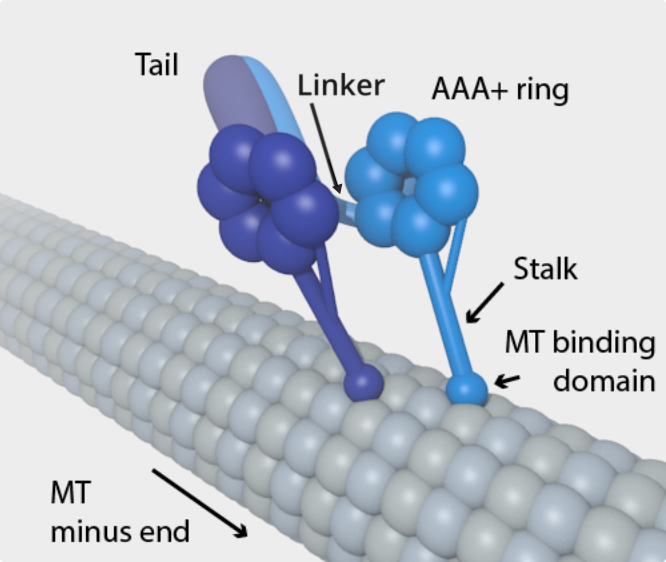
\includegraphics[width=0.6\columnwidth]{Figures/dynein_on_MT.png}
	\caption[Dynein on Microtubule]{\textbf{Dynein on Microtubule} Artist’s illustration of a dimer of cytoplasmic dynein heavy chains bounded to microtubule. This rendition similarly illustrates dynein’s structure as a domain-rod system, where the unlabeled linker domain connects the two AAA+ domains to the tail. \cite{TheTrappistArt}}
	\label{fig:final_disp}
\end{figure}


\section{Functions}
\textit{Purpose in the cell. What does dynein do that helps the cell operate? It walks on microtubule towards minus end. It uses chemical energy from ATP hydrolysis to convert into mechanical energy to walk and transport cargo with information along the cell. }

\begin{figure}[H]
	\centering
	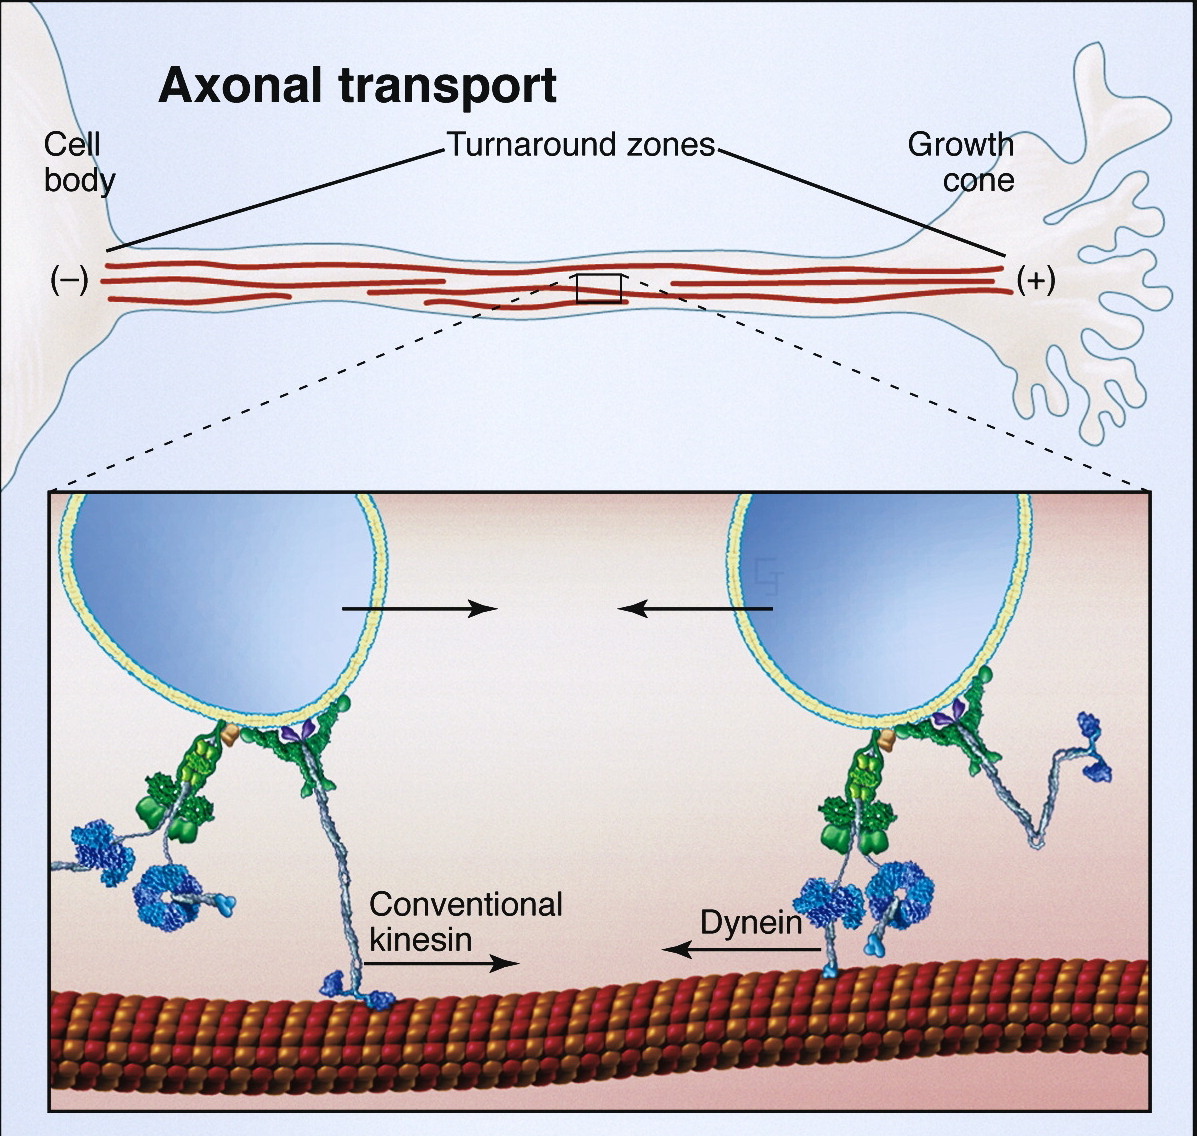
\includegraphics[width=0.6\columnwidth]{Figures/retrograde_transport.jpg}
	\caption[Retrograde Transport]{\textbf{Retrograde Transport} \cite{Vale2003molecular}}
	\label{fig:transport}
\end{figure}


\section{Architecture}
\textit{In-detail background knowledge on structure of dynein. Talk about each domain and their roles. Binding domain, six AAA+ domains, tail, and cargo. Stalk and linker that attaches things together. How the structure is so much larger than that of kinesin. dynein has flexibility because of its linker and in order to compensate for its huge domains. }

\begin{figure}[H]
	\centering
	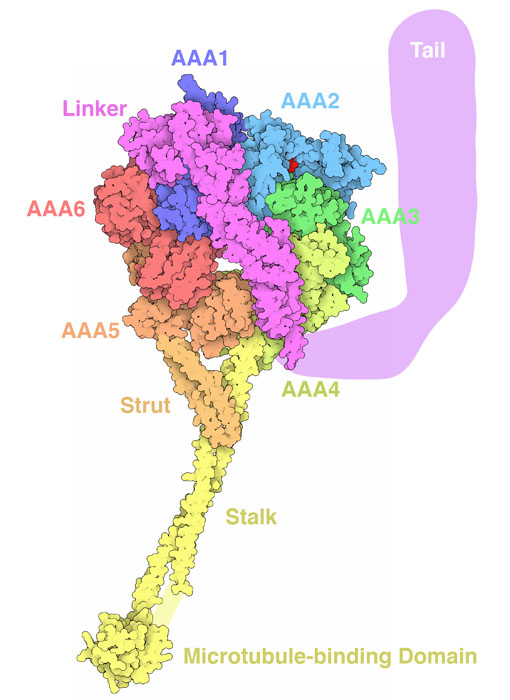
\includegraphics[width=0.6\columnwidth]{Figures/dynein_polypeptide.jpg}
	\caption[Polypeptide Structure]{\textbf{Polypeptide Structure} \cite{GoodsellArt}}
	\label{fig:polypeptide}
\end{figure}


\section{Stepping}
\textit{Biology and chemistry of stepping. What is actually causing it to step? ATP hydrolysis. Maybe short introduction on stepping and go more in detail in Power Stroke model. Say there are multiple theories and models of how dynein steps. Powerstroke, Winch, etc. Power stroke is most accepted. It can step on microtubule that is made up of tubulin dimers, $\alpha$ and $\beta$ tubulins. They are normally 8nm apart and so experimentalists believe dynein average step is always factor of 8nm. }


\begin{figure}[H]
	\centering
	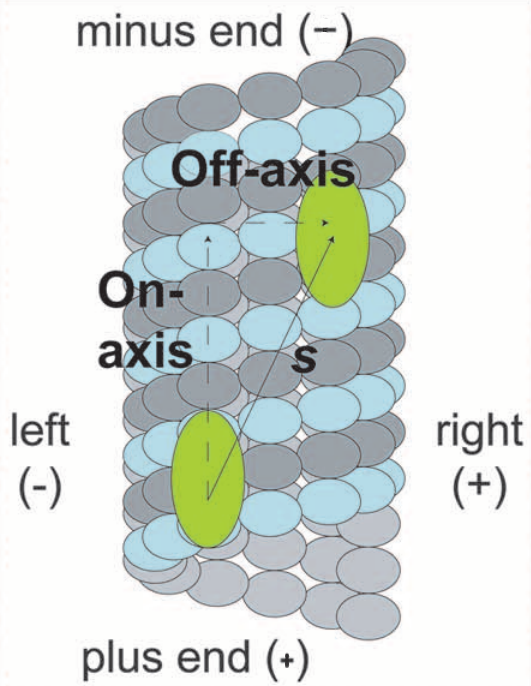
\includegraphics[width=0.3\columnwidth]{Figures/Onaxis.png}
	\caption[Stepping Axis]{\textbf{Stepping axis}  \cite{Dewitt2012} }
	\label{fig:YildizCorrelation}
\end{figure}


\subsection{Powerstroke Model}
\textit{Theorized model of stepping. Mechanochemical Cycle. Talk about ATP hydrolysis. Different conformational changes within a step. Look at linker and how it changes angles. Physically, it looks like it unbinds, stretches leg, then kicks forward, then diffuse back to MT.} 

\begin{figure}[H]
	\centering
	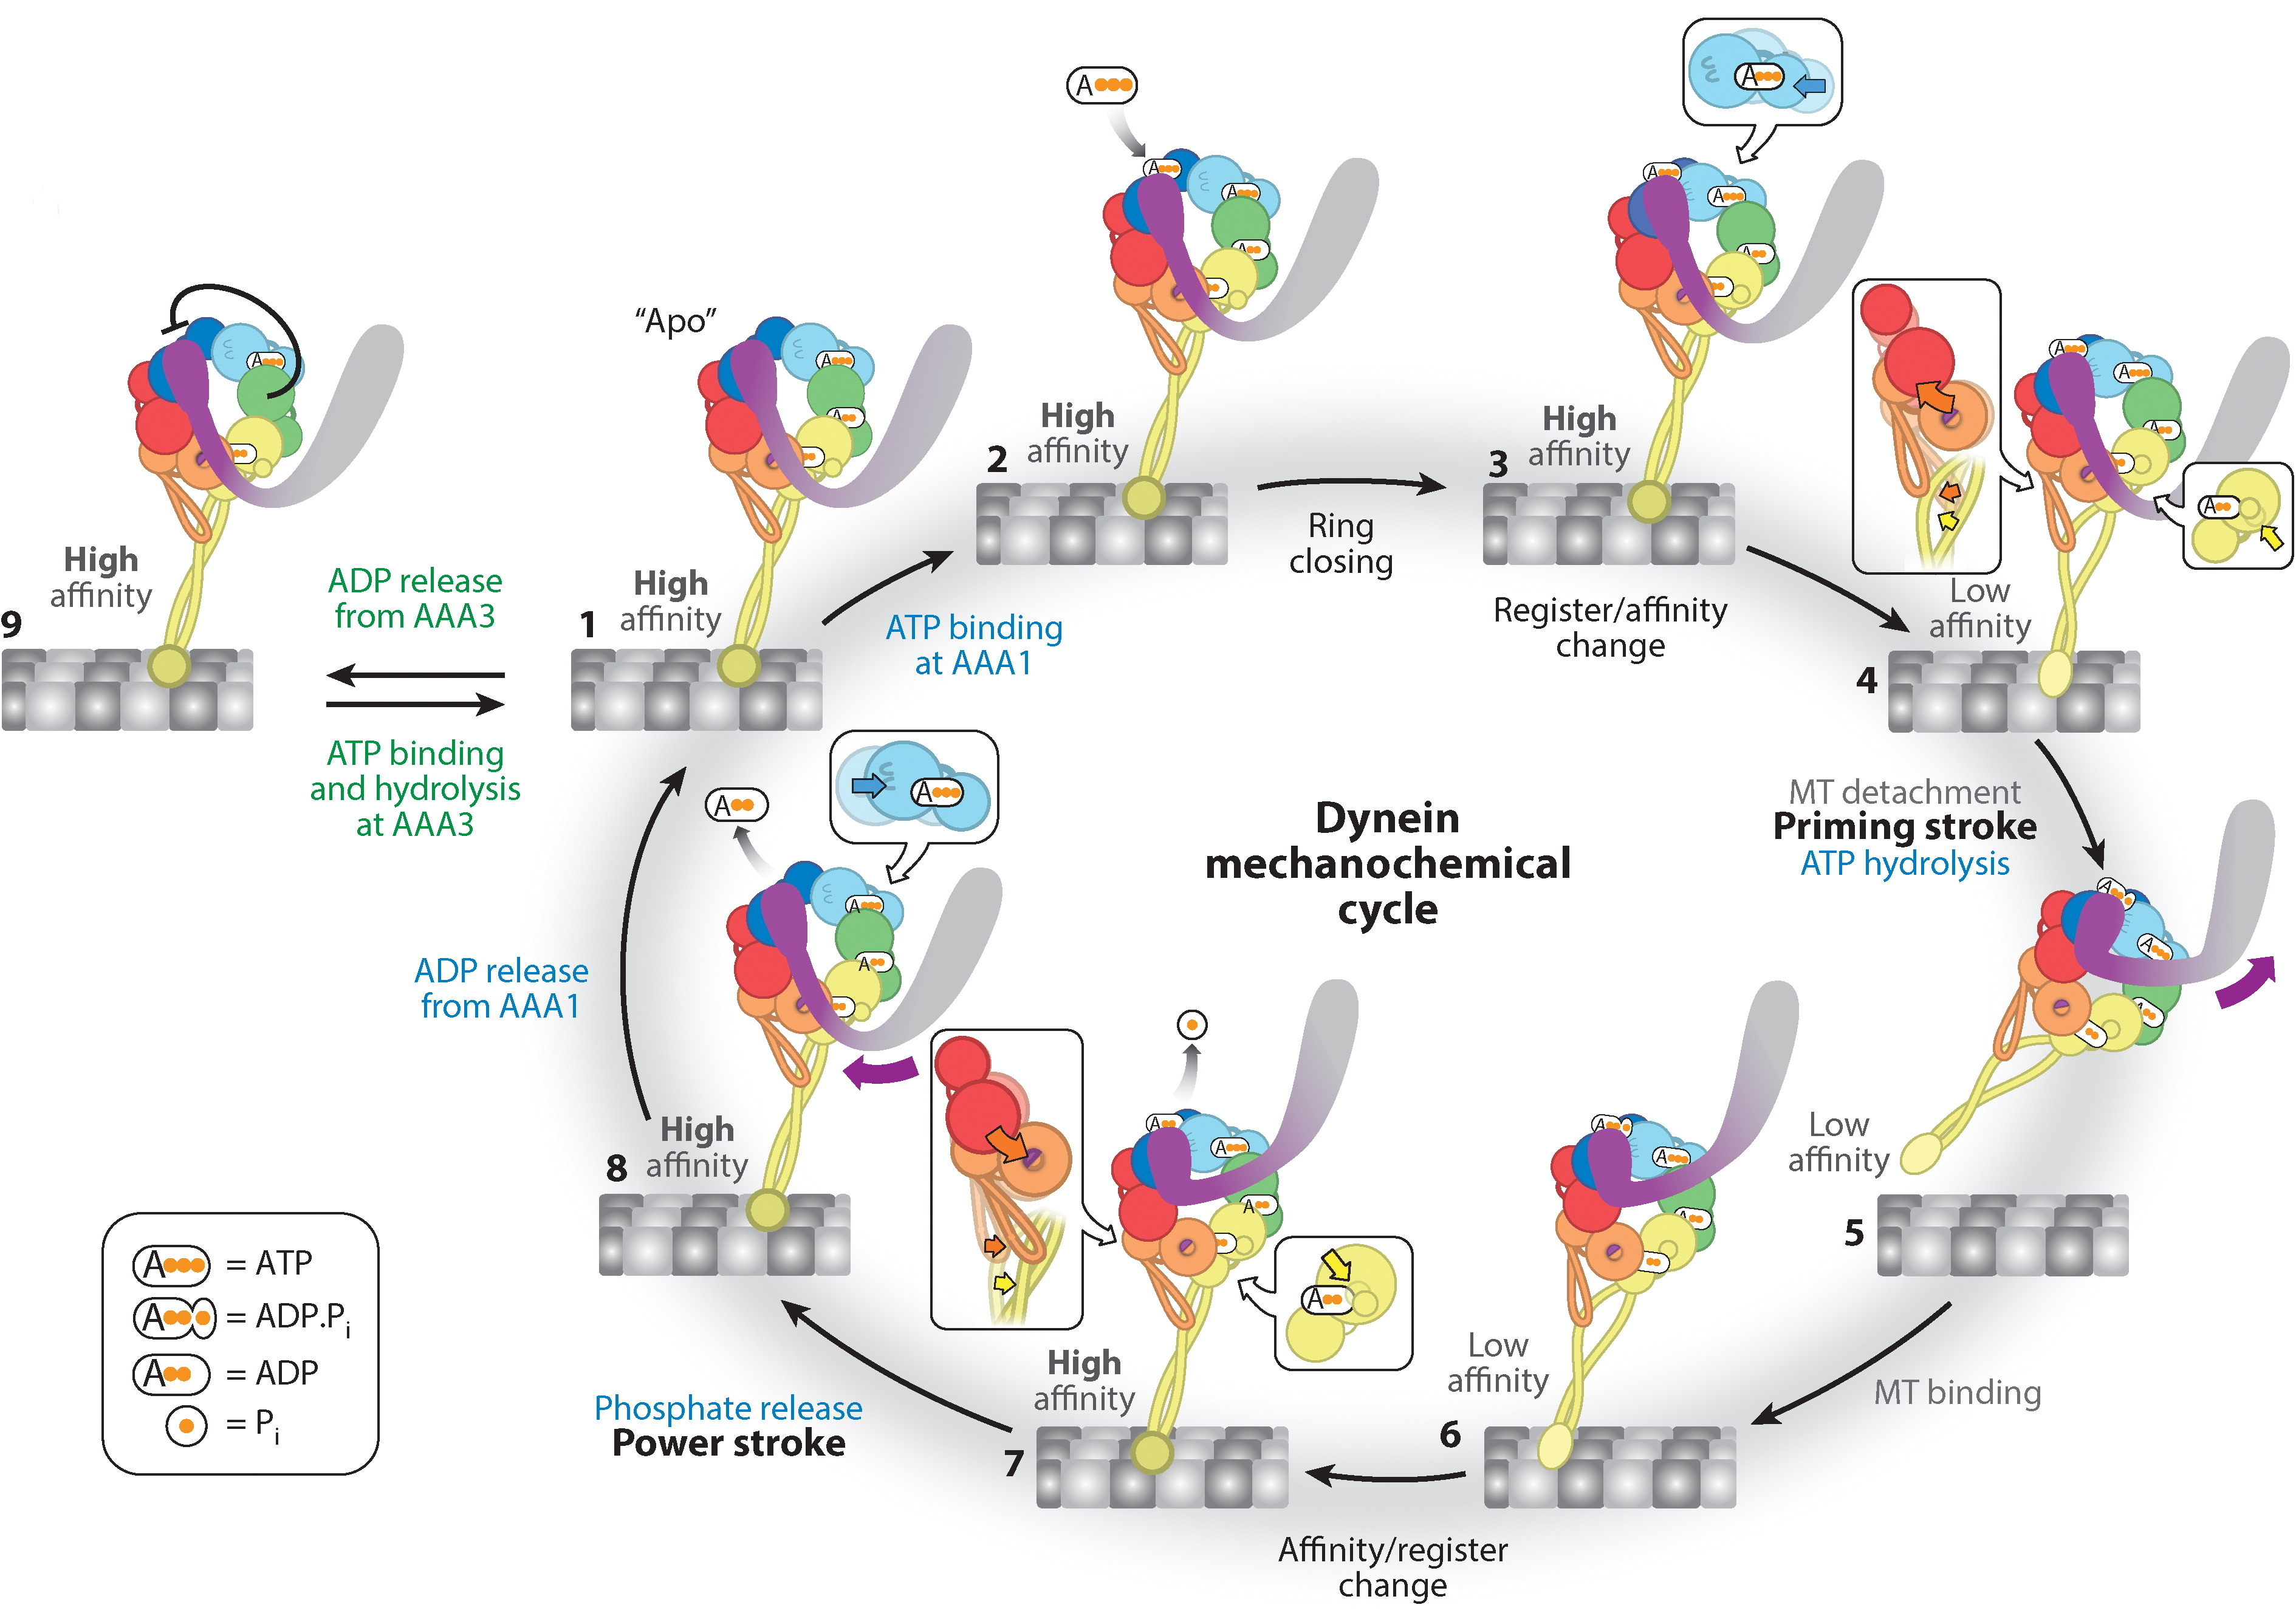
\includegraphics[width=1\columnwidth]{Figures/mechanochemical_cycle.jpeg}
	\caption[Mechanochemical Cycle]{\textbf{Mechanochemical Cycle}  \cite{Cianfrocco2015mechanism}}
	\label{fig:MechanochemicalCycle}
\end{figure}

\begin{figure}[H]
	\centering
	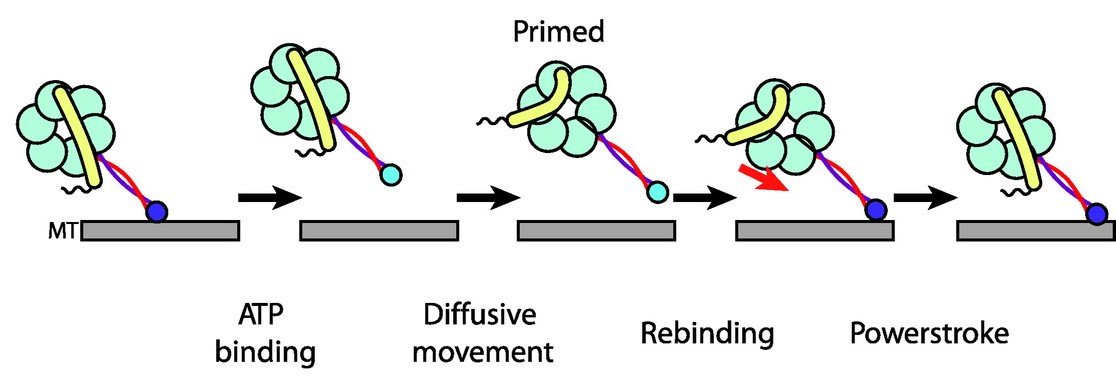
\includegraphics[width=1\columnwidth]{Figures/powerstroke.jpeg}
	\caption[Powerstroke]{\textbf{Powerstroke}  \cite{Carter2010communication} }
	\label{fig:Powerstroke}
\end{figure}


\section{Experimental Research on Dynein}
\textit{Most likely just short sections on experiments done on dynein.}
\subsection{Measuring}
\textit{How are experimentalists measuring dyneins stepping? Quantum dots on motor domains or quantum rod on tail, etc. }

\subsection{Interhead Coordination}
\textit{Purpose of my research. Trying to make model and fit to Yildiz analysis of dynein having interstep correlation. Dependency between step length and initial inter head separation.}

\begin{figure}[H]
	\centering
	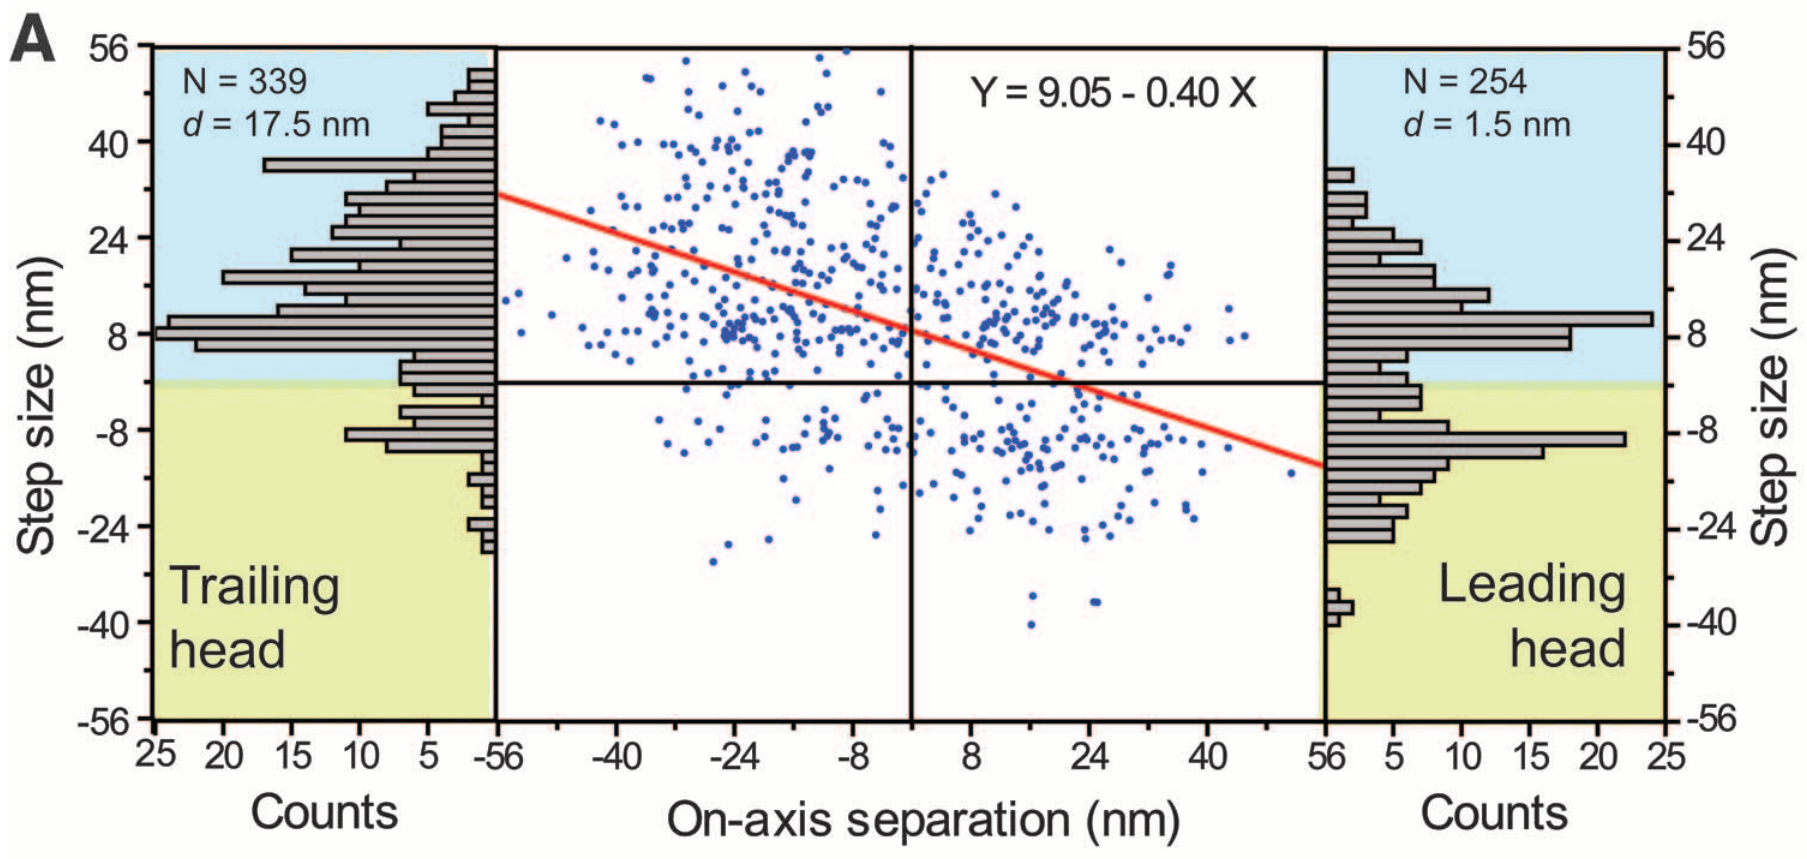
\includegraphics[width=1\columnwidth]{Figures/Yildiz_stepping.png}
	\caption[Stepping Correlation]{\textbf{Stepping Correlation}  \cite{Dewitt2012} }
	\label{fig:YildizCorrelation}
\end{figure}

	\chapter{Theory}
	\section{Model}
In order to reliably reproduce experimental observations of dynein's stepping, a model of dynein should responsibly conserve dynein's spatial information and complex structure under an aqueous environment. Doing so computationally introduces a strict balance between model accuracy and computational efficiency. In an attempt to best satisfy this difficult balance, we propose a coarse-grained model of dynein under a series of assumptions that benefits quick simulations of dynein taking a step. 


\subsection{2D Rigid Rod Model}
Since our goal is to investigate dynein's inter-step correlation during its forward directed stepping, we decided to model dynein as a 2-dimensional system of circular domains held together by massless rigid rods. These domains entitle two binding domains, two motor domains, and one tail domain, where each domain act as independent angular springs with their own spring constants.

\begin{figure}[H]
	\centering
	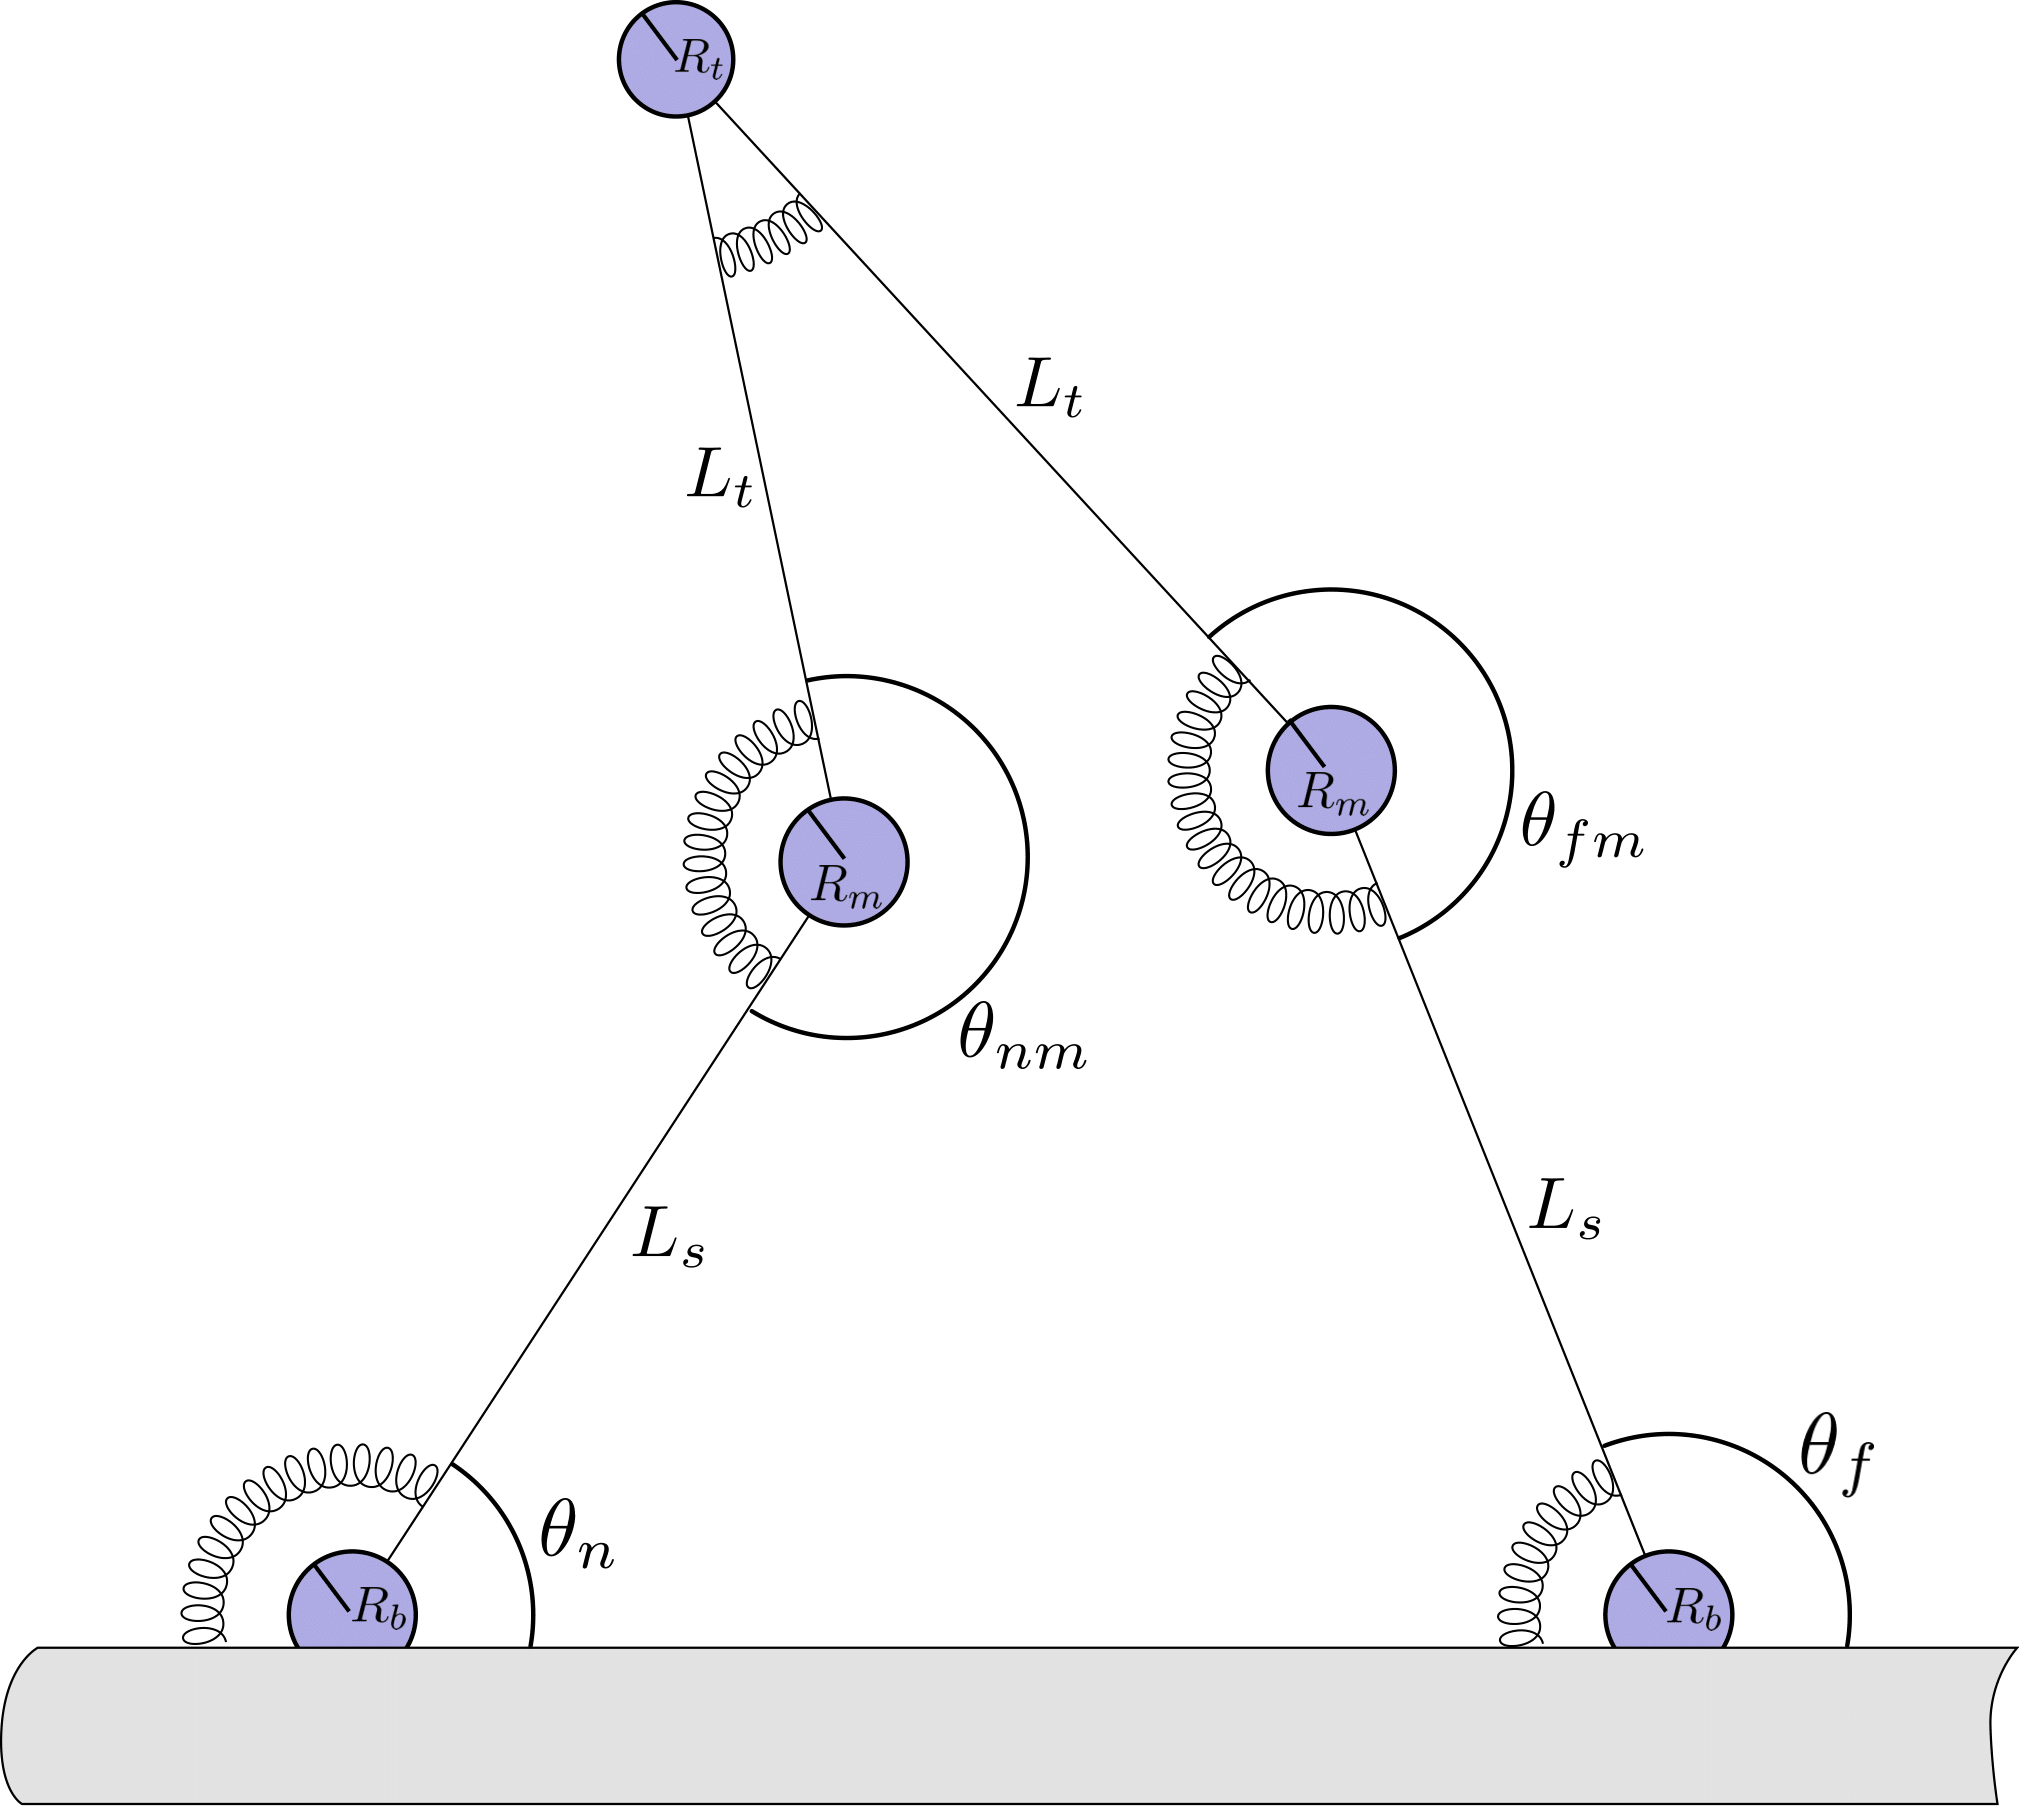
\includegraphics[width=0.6\columnwidth]{Figures/model-cartoon.png}
	\caption[Dynein Model]{\textbf{Dynein Model} \cite{Capek2017}}
	\label{fig:model}
\end{figure}

Despite dynein's complexity allowing its step to vary in both length and direction, we limit our model to one direction to eliminate a dimension (the off-axis) when analyzing the forward stepping pattern of dynein. This would also simplify the asymmetry of the microtubule when the dynein is stepping either on the $\alpha$ or $\beta$ tubulin. We also simplify the stalk and linker to be massless because we are assuming the drag force to be much larger than the mass of the rods and domains. The reasoning for this will be later discussed in Section \hyperref[sec:BrownianDynamics]{3.3} when we introduce Brownian dynamics. Although the stalk and linker of real dynein definitely have mass, we counteract the loss of interactions the rods experience with its environment by increasing the radii of the domains to be slightly larger than experimental measurements.

\subsection{Domains as Angular Springs}
In order to best simulate the stretching and forward kicking motion of the power stroke, we defined our domains to act as springs with spring constants $c_b$, $c_m$, and $c_t$ -- one for each respective domain. This can be analogous to how humans walk using their knees and ankles to bend and stretch accordingly when taking a step. Defining our domains as springs will allow us to influence forward bias walking by introducing a restoring force in each domain using Hooke's law: 
\begin{equation}
    F_i=-c_i(\theta_i-\theta_{i,eq})
\end{equation}
where $c_i$ is the spring constant, $\theta_i$ is angle corresponding to the $i^{th}$ domain, and $\theta_{i,eq}$ is the equilibrium angle in which biases the motion. Using this, we can calculate the energy of each domain by integrating and arriving to the familiar equation for spring energy.
\begin{equation}
    U_i=\frac{1}{2}c_i(\theta_i-\theta_{i,eq})
\end{equation}
Since dynein is symmetric for each heavy chain leg, the equilibrium angle will be identical for both binding and motor domain pairs, i.e. $\theta_{b,eq}$ is defined as the equilibrium angle for both binding domains, while $\theta_{m,eq}$ is defined as the equilibrium angle for both motor domains. This equation would then be used throughout the entirety of the simulation to determine the total energy of our dynein at a given conformation. 


\subsection{Two-State System}
According to the Mechanochemical Cycle (\hyperref[fig:MechanochemicalCycle]{Figure 2.5}), dynein can be in eight states over the course of a single step. However, many of these states possess similar conformations, where the dynein has either one binding domain bounded with the other diffusing above the microtubule or both binding domains bounded. Since the states that take the most time are during binding and unbinding \cite{}, we categorized the cycle into two main conformations: the pre-stroke one bound state and the post-stroke both bound state.

\begin{figure}[H]
	\centering
	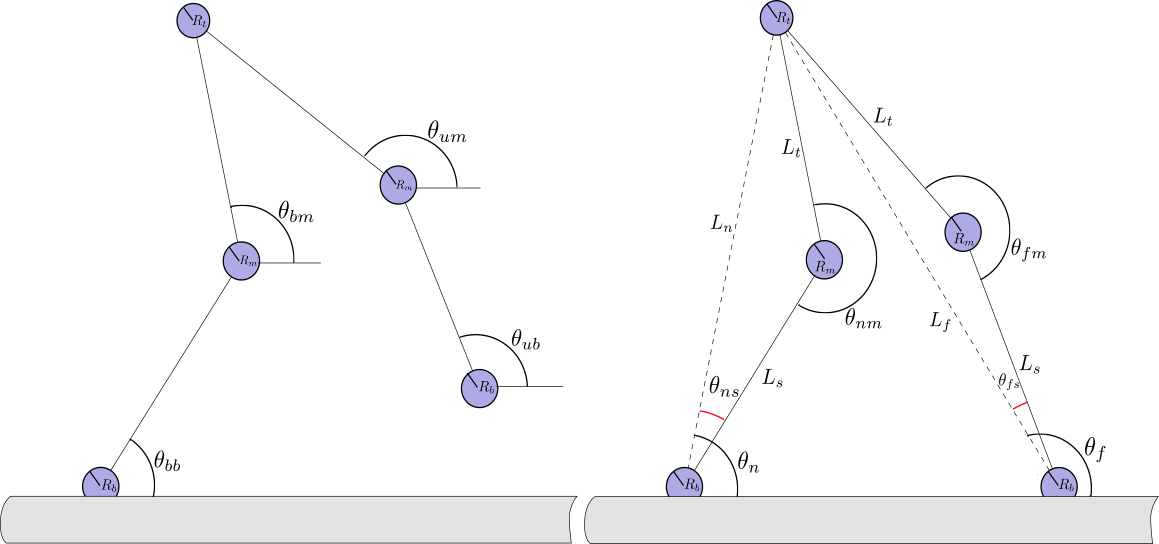
\includegraphics[width=0.8\columnwidth]{Figures/OB_vs_BB.PNG}
	\caption[One Bound vs. Both Bound]{\textbf{One Bound vs. Both Bound} Figure on left: Prestroke one bound state with labeling scheme ‘bounded’ and ‘unbouded’ for bounded leg and unbounded leg. Figure on the right: Poststroke both bound state with labeling scheme ‘near’ and ‘far’ for identifying heavy chain subunits \cite{Capek2017}.}
	\label{fig:final_disp}
\end{figure}

Differentiating the two allows us to more conveniently bias the conformational change by defining different equilibrium angles for both states.  


\subsection{Transitioning Between States}
\textit{Physics about conformational energy changes. How we model transitioning between BB state and OB state using transitioning rates and spring energies.}


\section{Simulation}
\textit{Pulled from Methods section. Maybe add a little intro to simulation process}
\par
These quick simulations are governed by a Monte Carlo algorithm, while the movement of the model is dictated by equations of motion describing domains interacting with a force of drag and a random force. This type of molecular simulations are more commonly known as Brownian dynamics. (\textbf{Possible take out sentence introducing MC and Brownian dynamics for later})


\subsection{Monte Carlo Algorithm}
\textit{Physics background on Monte Carlo. Stat Mech. }


\subsection{Brownian Dynamics}
\label{sec:BrownianDynamics}
\textit{Physics background on Brownian dynemaics. Newton's second law. What forces will we use? How do we determine the random force? etc.}

\subsection{Equations of Motion}
\textit{Derived equations of motion for each domain of our dynein from Brownian dynamics.}


\textit{STRAIGHT FROM PROPOSAL. FIXME}


Our entire model of dynein will be coded with a combination of both Python and C++. The structural features of dynein will be captured with a two-dimensional geometric model of circular domains connected by rigid rods. The dynamics of dynein will be captured by imposing both equilibrium and Brownian forces on each circular domain of the model, while the chemical properties will be modeled by sporadically transitioning between two states: a poststroke both bound state, and a prestroke one bound state. These two states are shown below in Figure 2.

The simulation for stepping will consist of running multiple independent steps that starts in a both bound configuration and transitions into the Brownian dynamics one bound state. In this state, each domain will undergo Brownian forces until the unbounded leg diffuses back onto the microtubule, thus completing a step. The Brownian dynamics only affects the one bound state since that is the only time (in our model) the domains undergo molecular interaction with its surroundings to achieve processive motion. This Monte Carlo method of collecting an ensemble of statistics after many simulations will lead to probability distributions of measured variables that can be compared with experimental results. The common experimental results analyzed in this field are the distribution of step lengths (defined as the final displacement of the “stepping” leg minus the initial displacement), stepping times, probability of the binding domain unbinding, and the velocity of a step. Once sufficient data is collected for each listed variable, plotting scripts on Python will be used to visualize the possible relationships between these variables and generate analysis for our model’s stepping patterns. Currently, a paper published by Dr. Ahmet Yildiz from the University of Berkeley proposed a possible relationship within dynein’s stepping, implying inter-step correlation [3]. Our model aims to reproduce these results by finding a set of parameters that matches Yildiz’s observation in the form of a linear regression of the step lengths against the initial binding domain separation. We hope to either support Yildiz’s claim or infer some new property of dynein that generated Yildiz’s observation.
	\chapter{Methods}
	\textit{All code for simulation can be accessed from GitHub through this link:}


\section{Simulation}
\textit{Picking Random angles to create random distribution of dynein configurations. Make sure to clarify that the simulation is split into two parts, the monte carlo both bound and brownian one bound. It is done this way in order for MC to generate ensemble of data rather quickly.}\\
\textit{Include a flow chart.}



\section{Time Evolution}
\textit{Simulate over a delta t during one bound and every iteration check for rebinding. How are the probabilities of binding and unbinding affected by the time.}

\section{Constants}
\textit{How we defined our constants based on experiment and pictures.  Need to include figures here of experiment dynein and how we measure the pre and post stroke equilibrium angles.}

\section{Parameter Fitting}
\textit{How we will fit our parameters to agree with Yildiz' experimental data of dynein stepping.}

\subsection{Rate Constants}
\textit{Fitting our rate constants were a huge part of our model and how we made sure our dynein can match experimentalist results.}

\section{Model Validation}
\textit{Any tests of our model to make sure the code is reasonably sound and that the physics makes sense. Make sure there is no bugs in code. What was the bug testing procedure.}

	\chapter{Results \& Discussion}
	\section{Optimized Parameters}
\textit{Talk about best-fit parameters that matched experimentalists data. Include table with all parameters.}
kekw
\section{Stepping Patterns}
\begin{figure}[H]
	\centering
	\includegraphics[width=0.7\columnwidth]{../../plots/mc_plots/u_final_disp_probability_distribution_30.0_5.50e+09_1.00e+08_0.2_1.05_0.0_90.0_197.0_242.0}
	\includegraphics[width=0.7\columnwidth]{../../plots/mc_plots/u_step_length_1d_probability_density_30.0_5.50e+09_1.00e+08_0.2_1.05_0.0_90.0_197.0_242.0}
	\caption[Final Displacement Probability Distribution]{\textbf{Stepping Probability Distribution Plots.} \textit{Top:} Two dimensional heatmap of binding domain displacement before and after a stepping cycle. Displacement is defined as the unbounded binding domain x position minus the binded binding domain x position, calculated before and after a step. Linear regression of the probability distribution indicates a dependence the final displacement of the step and its initial displacement, similarly to experiment. \textit{Bottom:} One dimensional probability density of step length. Step length defined as final displacement minus the initial displacement. Model compared to two experimental figures of stepping patterns from \citep{Dewitt2012}.} 
	\label{fig:final_disp}
\end{figure}

%\begin{figure}[H]
%	\centering
%	\includegraphics[width=0.7\columnwidth]{../../plots/mc_plots/%u_step_length_1d_probability_density_30.0_5.50e+09_1.00e+08_0.2_1.05_0.0_90.0_197.0_242.0}
%	\caption[Step Length Histogram]{\textbf{Step Length Histogram}}
%	\label{fig:step_length}
%\end{figure}

\begin{figure}[H]
	\centering
	\includegraphics[width=0.7\columnwidth]{../../plots/mc_plots/prob_lagging_vs_init_L_-0.3563}
	\caption[Probability of Lagging Step]{\textbf{Probability of Lagging Step}}
	\label{fig:step_length}
\end{figure}

\textit{Analysis on stepping patterns and what the parameters of our model indicate. Does dynein take a lot of fast steps?}

\section{Agree with Experiment?}
\textit{Whole point of parameter fitting was to agree with Yildiz and/or other experimental data. Did we do a good job?}
	\chapter{Conclusion}
	\section{Findings}
\textit{What do our results indicate? Do we think our model correctly represents real dynein and its stepping patterns?}


\section{Further Work}
\textit{How can we improve our model?}


\newpage
\cite{Burgess2003} \cite{Cianfrocco2015mechanism} \cite{Dewitt2012} \cite{Capek2017}
\bibliographystyle{unsrt}
\bibliography{references}


\end{document}
